\section{Python Visualization}
\subsection{Python IQ Data Visualization}
    In this experiment, We used Python 'matplotlib.pyplot.specgram' fucntion for IQ data visualization.
    In given file there are total 383 datasets of IQ data, so we could get 383 spectrogram images. \\
    \vspace{-4mm}  
    \begin{figure}[!h]\centering
    \hspace{15mm}
		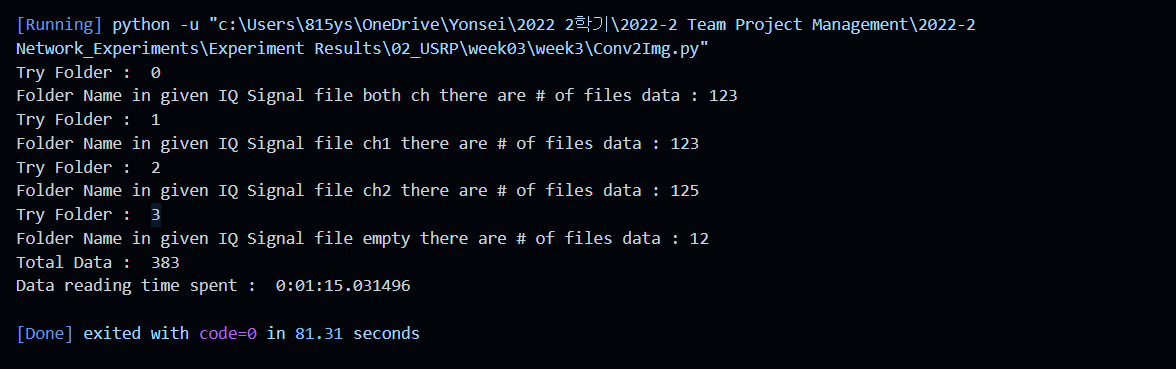
\includegraphics[width=.85\textwidth]{image/week03/1-2-1.png}
		\caption{\footnotesize IQ data visualization result}
		\vspace{-10pt}
    \end{figure}
%     \vspace{-4mm}  
%     \begin{figure}[!h]\raggedleft
%     \hspace{15mm}
% 		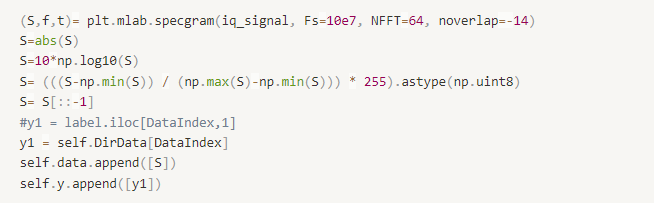
\includegraphics[width=.95\textwidth]{image/week03/1-1-1.png}
% 		\caption{\footnotesize Pyhton spectrogram function}
% 		\vspace{-10pt}
%     \end{figure}
    % The paramenters used in this function are \\
    % Fs : The sampling freqeuncy used to calculate the Fourier frequencies. \\
    % NFFT : The number of data points used in each block for the FFT.\\
    % noverlap : The number of points of overlap between blocks.\\
    
    \vspace{-4mm}  
    \begin{figure}[!h]\centering
    \hspace{15mm}
		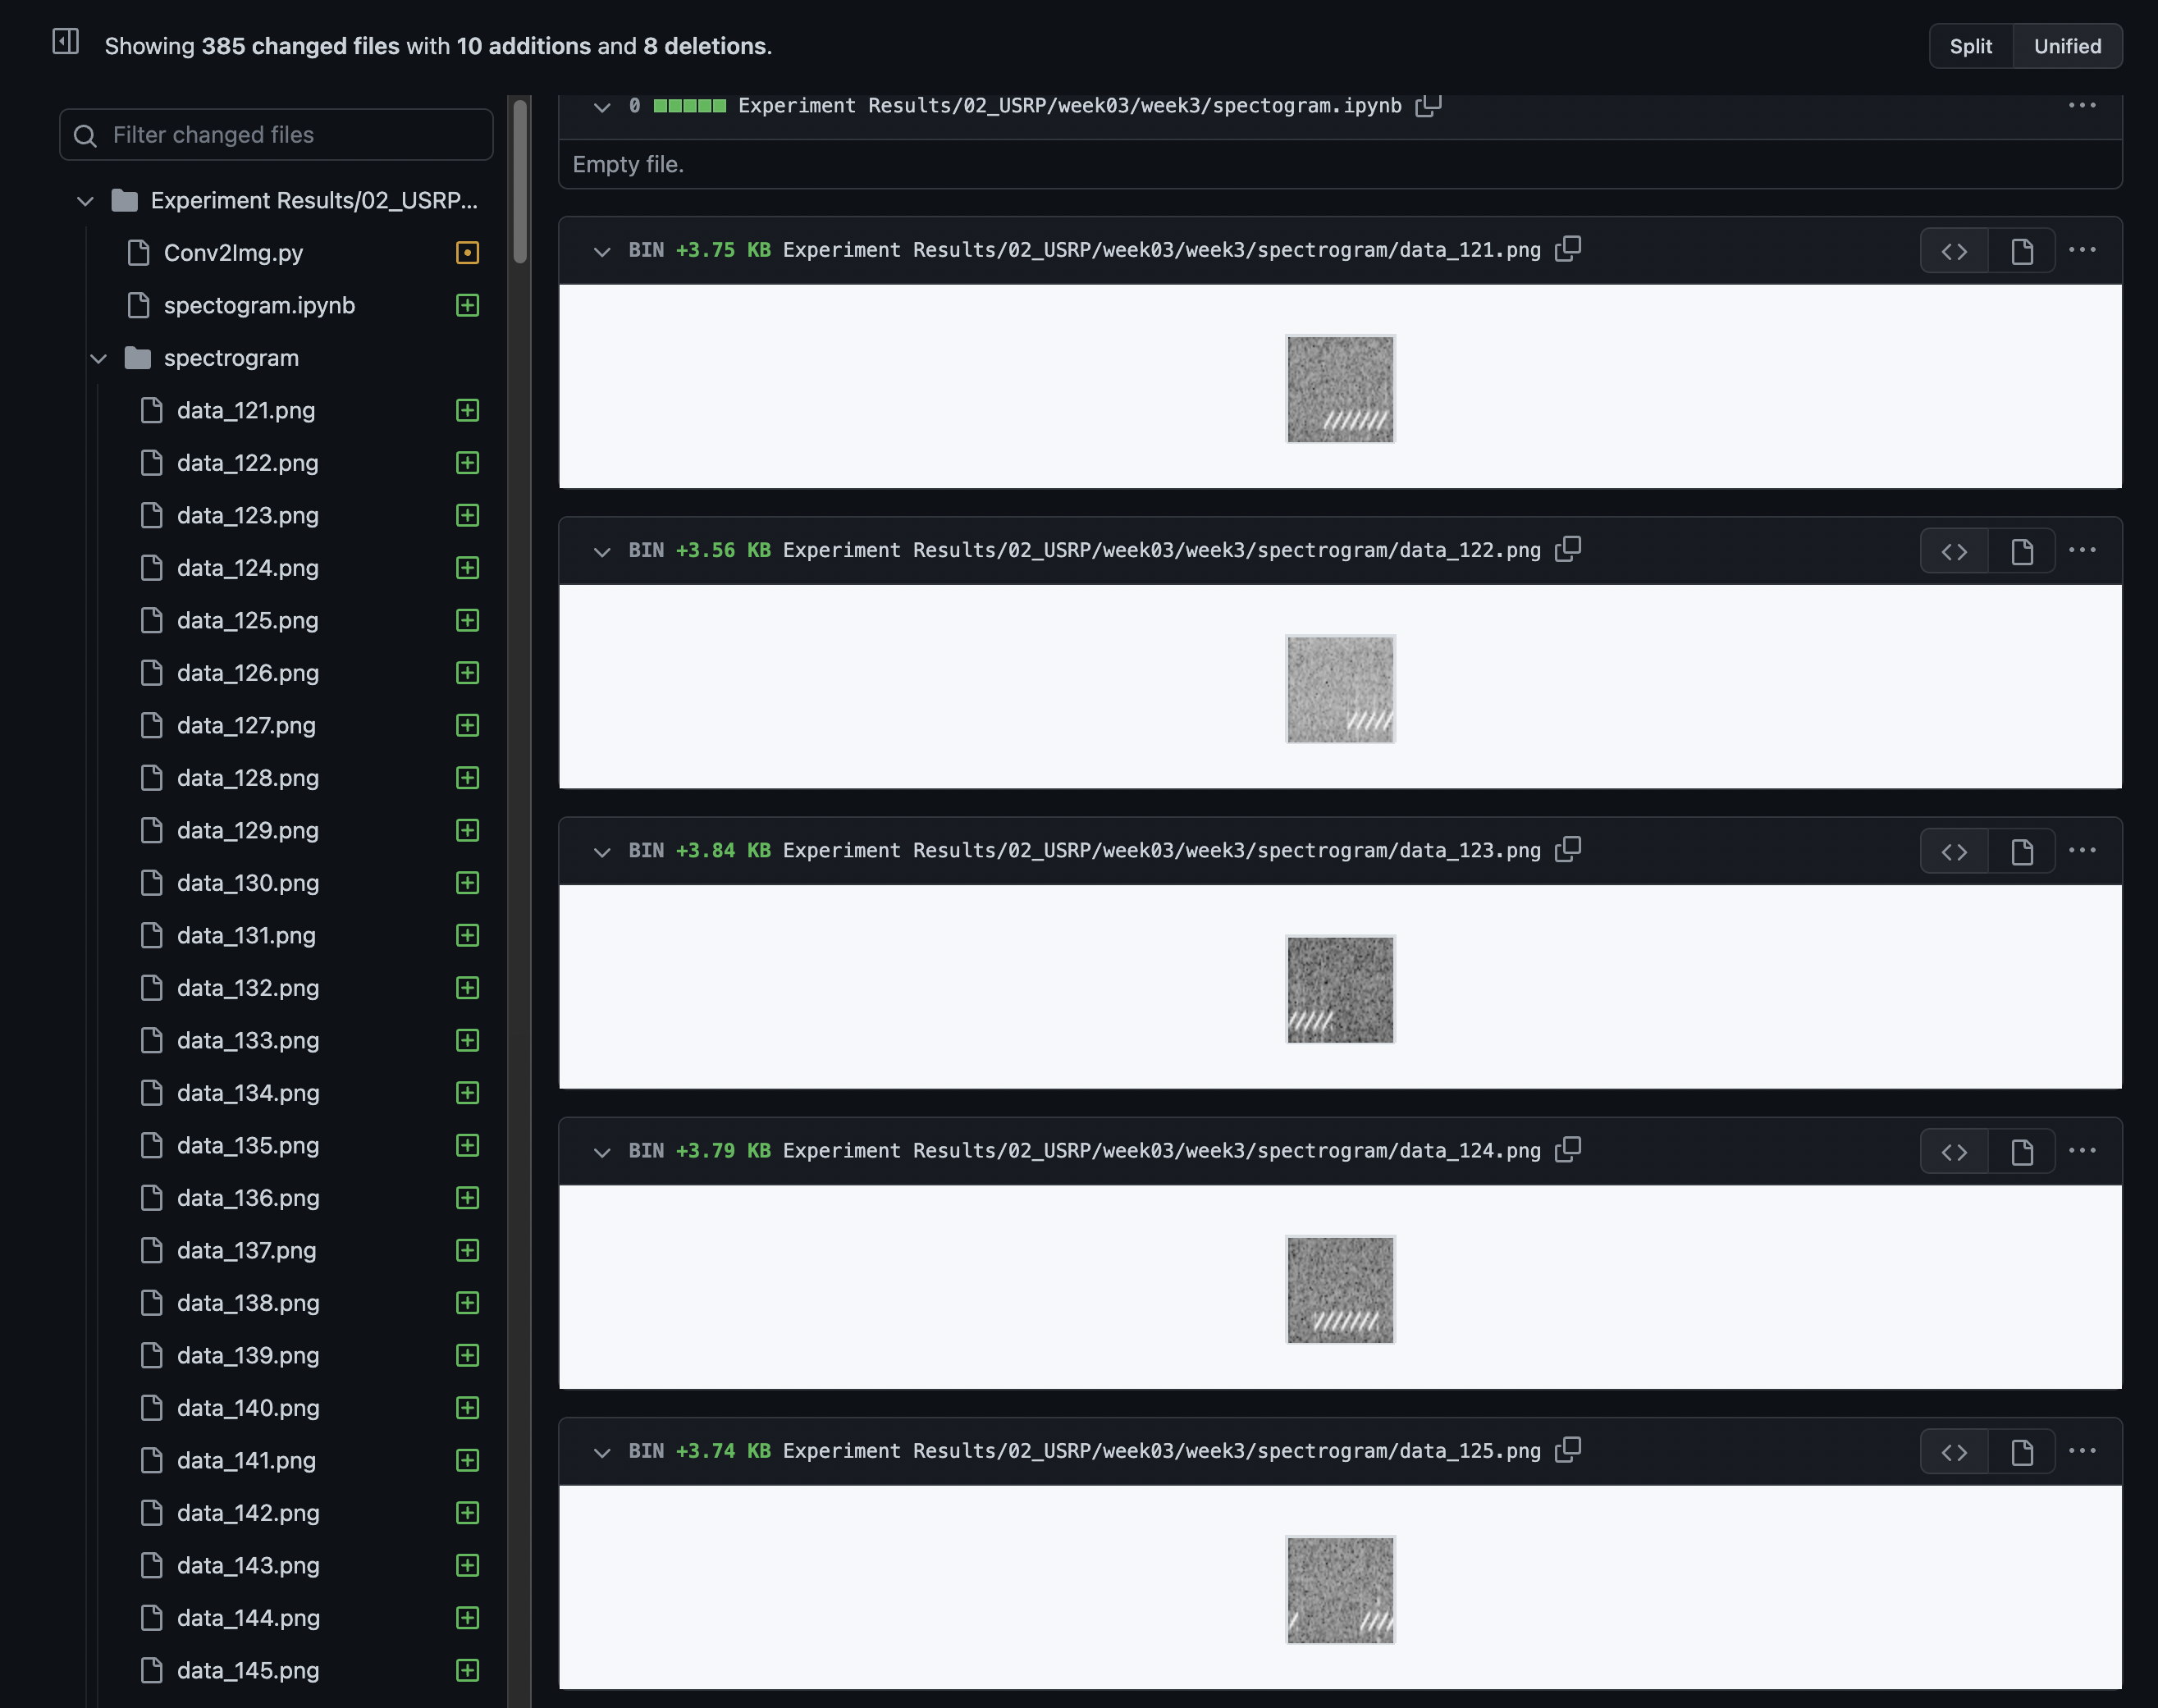
\includegraphics[width=.85\textwidth]{image/week03/bla.png}
		\caption{\footnotesize IQ data visualization result}
		\vspace{-10pt}
    \end{figure}
\clearpage